%----------------------------------------------------------------------------------
% Arquivo principal do TCC usando a classe tcc.cls
%----------------------------------------------------------------------------------

\documentclass[portuguese,oneside]{tcc}

% Pacotes adicionais (a classe já carrega vários por padrão)
\usepackage{graphicx}
\usepackage{pgfplots}
\usepackage{tikz}
\usetikzlibrary{positioning,shapes.geometric,shapes.misc,arrows.meta,fit}
\pgfplotsset{compat=1.18}
\usepackage{multirow}
\usepackage{nicefrac}
\usepackage{algorithmic}
\usepackage{hyphenat}
\usepackage[shortcuts]{extdash}
\newcommand{\safeincludegraphics}[2][]{%
  \IfFileExists{#2}{\includegraphics[#1]{#2}}{%
    \fbox{\parbox[c][0.3\linewidth][c]{0.6\linewidth}{\centering Imagem não disponível\\\texttt{\detokenize{#2}}}}%
  }%
}

%----------------------------------------------------------------
% Autor e metadados
%----------------------------------------------------------------
\author{Leonardo Preczevski Ramos}

\title{Dashboard Financeiro}
      {Financial Dashboard}

% Tipo de trabalho
%\tipotrabalho{\ptci}
%\tipotrabalho{\tci}
\tipotrabalho{\tcii}

% Curso
%\curso{\cc}
\curso{\si}
%\curso{\es}

% Orientação
\orientador{Ana Paula Terra Bacelo}
%\coorientador{Ciclano de Farias}

%----------------------------------------------------------------
\begin{document}

%----------------------------------------------------------------
% Dedicatória e epígrafe
%----------------------------------------------------------------
\dedicatoria{Dedico este trabalho aos meus pais, que sempre estiveram ao meu lado em todos os momentos.
Em especial ao meu pai, que passou a vida trabalhando em sua oficina de chapeação e pintura,
dedicando suas mãos ao ofício com esforço e dignidade, para que eu pudesse construir um futuro diferente.
Este diploma é tão deles quanto meu.}

\epigrafe{The best way to predict the future is to invent it.}{Alan Kay}

%----------------------------------------------------------------
% Agradecimentos (opcional)
%----------------------------------------------------------------
\begin{agradecimentos}
Agradeço aos meus pais, pelo suporte constante, esforço e dedicação incansáveis — pilares que sustentaram minha trajetória.
À minha família e amigos, que sempre acreditaram em mim mesmo quando as dificuldades pareciam maiores que os resultados.

Sou grato também aos colegas e professores que, de alguma forma, contribuíram para meu crescimento acadêmico e pessoal ao longo da graduação.
Cada troca, desafio e conversa teve seu valor neste caminho de aprendizado.
\end{agradecimentos}

%----------------------------------------------------------------
% Resumo e Abstract
%----------------------------------------------------------------
\begin{resumo}{educação financeira, planejamento pessoal, saúde financeira, autonomia econômica, validação com usuários}
Este trabalho apresenta o processo de concepção, desenvolvimento e validação do Dashboard Financeiro, solução digital criada para apoiar pessoas na organização de suas finanças diante do crescimento do endividamento no país. O texto contextualiza o problema, sintetiza as referências que embasam a proposta e descreve as decisões de produto que guiaram a experiência final: fluxo de acolhimento orientado, registro de receitas e despesas, categorização intuitiva, definição de metas e acompanhamento visual em painéis que integram indicadores, alertas e conteúdos educativos.
A pesquisa discute como as fases de levantamento de requisitos, prototipação, experimentação com usuários e acompanhamento com a banca orientadora direcionaram ajustes contínuos até a disponibilização pública da solução. Também são registradas as métricas coletadas, as validações conduzidas e as limitações encontradas, indicando caminhos para integrações automáticas com instituições financeiras e para o aprimoramento do monitoramento do produto. O resumo apresenta, portanto, uma visão abrangente da motivação, das entregas e dos próximos passos do projeto.
\end{resumo}

\begin{abstract}{financial education, personal budgeting, user validation, financial wellbeing, roadmap}
This work presents the conception, development, and validation of the Financial Dashboard, a digital solution designed to help people organize their finances amid rising household debt in Brazil. The document frames the social motivation, summarizes the theoretical references that support the proposal, and explains the product decisions that shaped the experience: guided onboarding, intuitive recording of income and expenses, category-based organization, goal setting, and visual panels that combine indicators, alerts, and educational guidance.
The research highlights how requirement gathering, prototyping, user testing, and faculty feedback steered continuous improvements until the solution became publicly available. It also records the metrics collected, the validations performed, and the limitations identified, pointing to future work such as automated connections with financial institutions and richer observability of user journeys. The abstract therefore offers a broad view of the motivation, outcomes, and next steps of the project.
\end{abstract}

%----------------------------------------------------------------
% Listas e Sumário (mantenha sem texto entre as linhas)
%----------------------------------------------------------------
\listoffigures       % (OPCIONAL)
\listoftables        % (OPCIONAL)
\listofalgorithms    % (OPCIONAL)
\listofacronyms      % (OPCIONAL)
\listofabbreviations % (OPCIONAL)
\listofsymbols       % (OPCIONAL)
\tableofcontents     % (OBRIGATÓRIO)

%----------------------------------------------------------------
% Capítulos (NÃO coloque conteúdo de capítulos aqui)
%----------------------------------------------------------------
\chapter{\label{chap:intro}Introdução}

\sigla{API}{Application Programming Interface}
\sigla{CRUD}{Create, Read, Update, Delete}
\sigla{HTTP}{Hypertext Transfer Protocol}
\sigla{IDE}{Integrated Development Environment}
\sigla{JPA}{Java Persistence API}
\sigla{JSON}{JavaScript Object Notation}
\sigla{PUCRS}{Pontifícia Universidade Católica do Rio Grande do Sul}
\sigla{REST}{Representational State Transfer}
\sigla{TCC}{Trabalho de Conclusão de Curso}
\sigla{UI}{User Interface}
\sigla{UX}{User Experience}

\abrev{VSCode}{Visual Studio Code}
\abrev{BD}{Banco de Dados}

\simbolo{$\pi$}{Constante com valor aproximado de 3{,}14}

Com o avanço acelerado da tecnologia e a popularização da internet, ferramentas digitais têm sido integradas de forma crescente ao cotidiano, impactando positivamente áreas como saúde, educação, mobilidade urbana e finanças pessoais. Essa digitalização viabiliza maior eficiência, automação de tarefas e acesso aprimorado à informação, promovendo mais controle e autonomia para o cidadão em suas tomadas de decisão.

No âmbito financeiro, observa-se o crescimento de plataformas digitais voltadas à gestão de recursos pessoais. O controle financeiro, que já foi visto como uma recomendação, é hoje uma necessidade premente diante do contexto econômico brasileiro. Em dezembro de 2024, o número de brasileiros endividados chegou a \textbf{73{,}51 milhões} \cite{SERASA2024}. Em janeiro de 2025, o percentual de famílias endividadas reduziu-se para \textbf{76{,}1\%}, queda de \textbf{0{,}6 p.p.} em relação a dezembro, embora o quadro permaneça preocupante \cite{PEIC2025}.

A saúde financeira dos brasileiros também apresentou leve melhora: o \textit{Índice de Saúde Financeira do Brasileiro} (I\hyp SFB), desenvolvido pela FEBRABAN em parceria com o Banco Central, subiu de \textbf{56{,}2} em 2023 para \textbf{56{,}7} em 2024 — o melhor resultado dos últimos três anos \cite{BCB2024,ISFB2024}. Complementando esse cenário, um levantamento indica que \textbf{cerca de 57 milhões} de brasileiros estão endividados sem perceber, e \textbf{19 milhões} já chegaram a negativar o nome, evidenciando a urgência de maior conscientização \cite{SERASA2025INFO}.

A má administração de recursos pode levar ao acúmulo de dívidas, perda de poder de compra e prejuízo à qualidade de vida. Por outro lado, uma gestão consciente viabiliza estabilidade, criação de reservas de segurança e o alcance de objetivos pessoais. A educação financeira, nesse sentido, emerge não apenas como ferramenta de empoderamento individual, mas também como base de decisões mais equilibradas e sustentáveis \cite{ANBIMA2024}.

Diante desse contexto, este trabalho apresenta o desenvolvimento e a implantação do \textbf{Dashboard Financeiro}, uma aplicação web voltada à gestão de finanças pessoais. Seu desenho \textit{full\hyp stack} organiza-se em duas camadas principais: o \textbf{frontend}, responsável pela interface e interação com o usuário; e o \textbf{backend}, responsável pela lógica de negócio, autenticação e persistência dos dados. Essa combinação modular favorece a criação de sistemas escaláveis e alinhados às boas práticas de engenharia de software.

O termo \textit{dashboard} refere-se a um painel visual que sintetiza dados e indicadores de forma clara e acessível, facilitando a identificação de padrões, o monitoramento de metas e a tomada de decisões embasadas \cite{MUNZNER2014,FEW2017}. No \textbf{Dashboard Financeiro}, o usuário registra transações, classifica receitas e despesas, define metas e acompanha visualizações que evidenciam comportamentos e tendências ao longo do tempo.

\section*{Objetivos}

\textbf{Objetivo Geral}

Desenvolver e implantar uma aplicação web \textit{full\hyp stack}, denominada \textbf{Dashboard Financeiro}, para organização e análise de finanças pessoais, utilizando práticas modernas, seguras, escaláveis e acessíveis de engenharia de software.

\textbf{Objetivos Específicos}

\begin{itemize}
    \item Permitir o registro e a categorização de receitas e despesas por meio de uma interface intuitiva;
    \item Apresentar gráficos e indicadores financeiros de forma dinâmica e responsiva;
    \item Oferecer recursos de definição de metas mensais e alertas de desempenho com notificações por e\hyp mail;
    \item Garantir segurança e privacidade dos dados por meio de autenticação baseada em tokens e criptografia;
    \item Estruturar a aplicação com arquitetura orientada a serviços e persistência em banco de dados relacional;
    \item Implantar a aplicação em ambiente de nuvem para acesso remoto e escalabilidade.
\end{itemize}

Todos os objetivos foram endereçados no volume atual: os capítulos~\ref{chap:chap3} e~\ref{chap:chap5} detalham a arquitetura orientada a serviços e a infraestrutura em produção, enquanto o Capítulo~\ref{chap:chap4} evidencia o cumprimento do cronograma e o Capítulo~\ref{chap:chap6} descreve a validação funcional e os próximos passos.

\section{Potencial de Impacto da Solução}

O \textbf{Dashboard Financeiro} visa transformar a forma como os usuários lidam com suas finanças, fomentando hábitos saudáveis e promovendo autonomia econômica. Sua abordagem educativa, visual e segura pode gerar impacto positivo na vida das pessoas — ajudando-as a planejar, economizar, evitar endividamentos desnecessários e tomar decisões mais conscientes, com efeitos benéficos para a sociedade como um todo.
 % Introdução
\chapter{\label{chap:chap2}Fundamentação Teórica}

Este capítulo apresenta os conceitos, fundamentos e tecnologias que embasam o \textbf{Dashboard Financeiro}. O objetivo é contextualizar teoricamente a escolha do tema, reforçar sua relevância e demonstrar como a aplicação se relaciona com a realidade econômica atual, com foco em educação financeira, visualização de dados (BI) e usabilidade.

\section{Educação Financeira e Controle Pessoal de Gastos}
A educação financeira é amplamente reconhecida como essencial para promover bem-estar econômico e social. Evidências recentes mostram uma lacuna entre a importância percebida do tema e sua prática cotidiana: a \textit{17ª edição do Observatório FEBRABAN} aponta que \textbf{55\%} dos brasileiros afirmam entender \textbf{pouco (40\%)} ou \textbf{nada (15\%)} de educação financeira, embora a maioria considere o tema relevante para a vida pessoal \cite{FEBRABAN2025}. Em paralelo, o \textit{Índice de Saúde Financeira do Brasileiro} (I-SFB) --- desenvolvido pela FEBRABAN com apoio do Banco Central do Brasil --- registrou \textbf{56{,}7 pontos em 2024}, o maior patamar dos últimos três anos, o que sugere leve melhora, ainda que em patamar moderado \cite{BCB2024,ISFB2024}.

Esses dados reforçam um diagnóstico: há espaço para soluções tecnológicas que traduzam conceitos financeiros em linguagem acessível e, ao mesmo tempo, ofereçam \textit{feedback} visual e orientações práticas. Bancos e \textit{fintechs} já incorporam funções de controle financeiro em seus aplicativos (p.\,ex., categorização automática e alertas), mas em geral essas ofertas:
\begin{enumerate}
    \item ficam restritas ao próprio ecossistema da instituição (usuários/clientes), reduzindo a interoperabilidade;
    \item priorizam a visão transacional (extrato/saldo) em detrimento de \textbf{recursos educativos} e de \textbf{insights} analíticos acionáveis;
    \item apresentam barreiras de custo para funcionalidades avançadas ou interfaces que não favorecem o aprendizado progressivo.
\end{enumerate}

O \textbf{Dashboard Financeiro} proposto neste trabalho busca preencher essa lacuna com uma abordagem \textbf{independente}, \textbf{inclusiva} e \textbf{educativa}, combinando:
(i) \textbf{acompanhamento} de receitas/despesas e metas;
(ii) \textbf{visualizações analíticas} que facilitam a interpretação (padrões de consumo, desvios, projeções);
(iii) \textbf{conteúdo instrucional embutido} (dicas, microexplicações e boas práticas).
Ao integrar \textit{visualização + orientação}, a ferramenta pretende aumentar a autonomia do usuário e apoiar a formação de hábitos financeiros saudáveis, alinhada às diretrizes e achados recentes sobre o tema \cite{ANBIMA2024}.

Os percentuais dessa autopercepção são sintetizados na Figura~\ref{fig:educacao_financeira_percepcao}, permitindo visualizar em um único painel como ainda predomina o entendimento limitado sobre educação financeira entre os brasileiros.

\vspace{0.5em}
\textbf{Visualização 1 — Autopercepção do conhecimento em educação financeira (dados reais).}

\begin{figure}[ht]
\centering
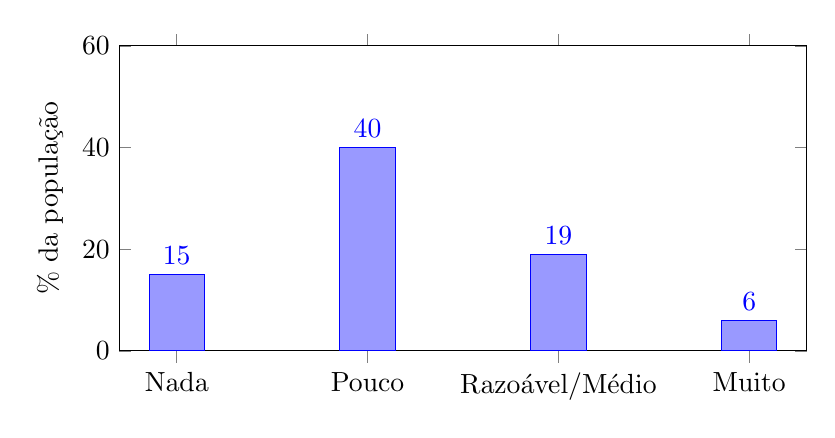
\begin{tikzpicture}
\begin{axis}[
    width=0.85\linewidth,
    height=0.45\linewidth,
    ybar,
    bar width=20pt,
    symbolic x coords={Nada,Pouco,Razoável/Médio,Muito},
    xtick=data,
    ylabel={\% da população},
    ymin=0, ymax=60,
    nodes near coords,
    nodes near coords align={vertical},
]
% FEBRABAN/IPESPE 2025: Nada 15, Pouco 40, Razoável/Médio 19, Muito 6
\addplot+[fill=blue!40] coordinates {
    (Nada,15) (Pouco,40) (Razoável/Médio,19) (Muito,6)
};
\end{axis}
\end{tikzpicture}
\caption{Autopercepção do conhecimento em educação financeira no Brasil (2025). \textbf{Fonte:} Observatório FEBRABAN/IPESPE \cite{FEBRABAN2025}.}
\label{fig:educacao_financeira_percepcao}
\end{figure}

\section{Visualização de Dados, Business Intelligence e Interface Analítica}
Transformar dados brutos em \textit{insights} compreensíveis é central em sistemas de apoio à decisão. Na literatura de visualização, boas práticas destacam \textbf{clareza}, \textbf{saliência do que importa} e \textbf{design parcimonioso} para leitura rápida e sem ambiguidade \cite{MUNZNER2014,FEW2017}. Em aplicações financeiras pessoais, a experiência do usuário (UX) e a usabilidade são determinantes para adoção e percepção de valor: interfaces bem projetadas reduzem carga cognitiva e encorajam decisões embasadas \cite{NIELSEN1994}.

No \textbf{Dashboard Financeiro}, a camada analítica está organizada como um \textbf{painel de BI pessoal} com:
\begin{itemize}
    \item \textbf{Controle de intervalo}: o usuário escolhe entre 7 dias, 30 dias, 6 meses ou 12 meses para filtrar toda a visão, permitindo comparar períodos curtos e longos sem sair da tela.
    \item \textbf{Cartões de síntese}: logo no topo são exibidos os totais de receitas, despesas, saldo líquido e saldo consolidado das contas, sempre considerando o intervalo selecionado e atualizados diretamente a partir dos dados reais registrados.
    \item \textbf{Evolução mensal e contas paginadas}: a seção ``Evolução mensal'' lista mês a mês quanto entrou e saiu e destaca se o resultado ficou positivo ou negativo, enquanto a coluna lateral mostra as contas bancárias cadastradas, com agência, número e saldo atual paginados em blocos de até quatro registros.
    \item \textbf{Categorias em destaque}: receitas e despesas são agrupadas por categoria, permitindo identificar rapidamente onde estão os maiores volumes por meio de cartões e gráficos que evidenciam o peso de cada área do orçamento.
    \item \textbf{Modo analítico interativo}: ao alternar de ``Quadros'' para ``Gráficos'', o painel revela comparações como a evolução do saldo por conta, o impacto percentual de cada categoria, o fluxo diário recente e as curvas de tendência de receitas e despesas com indicação do quanto cresceram ou caíram.
    \item \textbf{Monitoramento de metas}: o painel exibe quantas metas estão ativas, concluídas, ultrapassadas ou expiradas, além de barras de progresso individuais; metas com data final aparecem em uma tabela que avisa sobre prazos próximos ou vencidos.
\end{itemize}

A Figura~\ref{fig:isfb_serie} resume a trajetória recente do I-SFB para justificar por que o produto prioriza feedbacks contínuos sobre hábitos: mesmo com oscilações positivas, o indicador permanece apenas em nível moderado.

\vspace{0.5em}
\textbf{Visualização 2 — Série histórica recente do I-SFB (dados reais).}

\begin{figure}[ht]
\centering
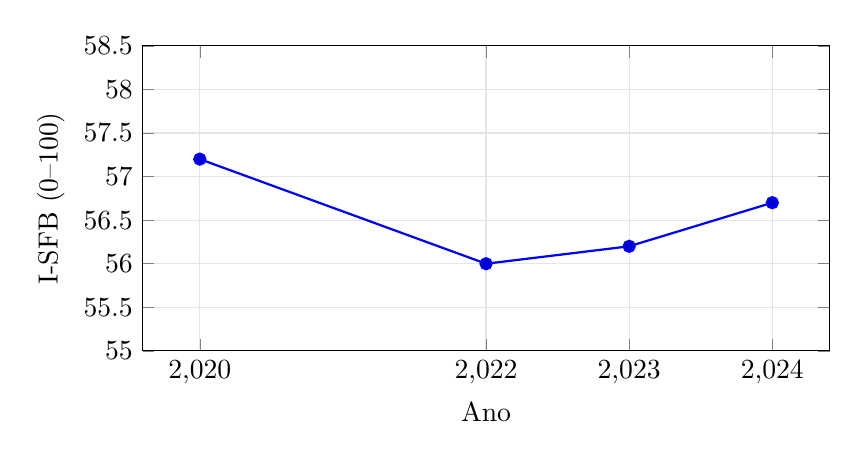
\begin{tikzpicture}
\begin{axis}[
    width=0.85\linewidth,
    height=0.45\linewidth,
    xlabel={Ano},
    ylabel={I-SFB (0--100)},
    ymin=55, ymax=58.5,
    xtick={2020,2022,2023,2024},
    ytick distance=0.5,
    grid=both,
    grid style={gray!20}
]
% Pontos (fontes citadas): 2020=57.2; 2022=56.0; 2023=56.2; 2024=56.7
\addplot+[mark=*,thick] coordinates {(2020,57.2) (2022,56.0) (2023,56.2) (2024,56.7)};
\end{axis}
\end{tikzpicture}
\caption{I-SFB: série recente (2020–2024). \textbf{Fontes:} FEBRABAN/BCB \cite{FEBRABAN2022,BCB2024,ISFB2024}.}
\label{fig:isfb_serie}
\end{figure}

A série histórica do \textit{Índice de Saúde Financeira do Brasileiro} (Figura~\ref{fig:isfb_serie}) evidencia por que o painel enfatiza feedbacks contínuos: mesmo com leve recuperação após 2022, o indicador permaneceu abaixo de 57 pontos, faixa classificada como ``atenção''. Essa fotografia nacional motiva recursos do Dashboard que acompanham evolução mensal, metas e categorias, ajudando o usuário a enxergar se suas finanças pessoais estão melhorando no mesmo período em que o país busca sair de um patamar apenas moderado de saúde financeira.

\section{Exemplos de Ferramentas Semelhantes e Oportunidades de Melhoria}
O mercado brasileiro possui diversas soluções de controle financeiro pessoal. A seguir, estruturam-se referências concorrentes ao \textbf{Dashboard Financeiro}, com uma visão comparativa de funcionalidades e uma descrição objetiva de cada uma.

\subsection{Guiabolso}\label{subsec:guiabolso}

O Guiabolso~\cite{GUIABOLSO2021} ficou marcado por integrar dados de múltiplas instituições financeiras por meio do acesso consentido às contas dos usuários, apresentando uma visão consolidada dos fluxos de entrada e saída. A plataforma combina sincronização automática com instituições bancárias, categorização assistida de lançamentos e recomendações baseadas em comportamento de gastos. Além da funcionalidade transacional, o aplicativo oferece trilhas de educação financeira e conteúdos editoriais voltados a crédito consciente, renegociação de dívidas e planejamento de metas.

% Substitua o caminho abaixo pela imagem real que você baixar
\begin{figure}[H]
\centering
\safeincludegraphics[width=0.75\linewidth]{figs/guiabolso.jpg}
\caption{Interface do aplicativo Guiabolso (ilustrativa).}
\label{fig:guiabolso}
\end{figure}

\subsubsection*{Guiabolso — Pontos fortes}
\addcontentsline{toc}{subsubsection}{Guiabolso — Pontos fortes}
\begin{itemize}
    \item Integração automática com contas bancárias, reduzindo a necessidade de lançamentos manuais;
    \item Categorização inteligente que aprende com os ajustes do usuário;
    \item Visão consolidada de transações, saldos e compromissos;
    \item Campanhas de renegociação que ajudam a reduzir dívidas com parceiros credenciados.
\end{itemize}

\subsubsection*{Guiabolso — Limitações}
\addcontentsline{toc}{subsubsection}{Guiabolso — Limitações}
\begin{itemize}
    \item Ênfase em ofertas de produtos financeiros, o que pode reduzir a percepção de neutralidade;
    \item Dependência do ecossistema institucional e das políticas de compartilhamento de dados;
    \item Recursos educativos concentrados em conteúdos estáticos, com menor orientação personalizada;
    \item Encerramento das operações no Brasil em 2021, sinalizando riscos de sustentabilidade para plataformas baseadas em open finance.
\end{itemize}

\begin{table}[H]
\centering
\caption{Guiabolso — síntese dos recursos avaliados.}
\label{tab:guiabolso_comparativo}
\begin{tabular}{p{0.37\linewidth}p{0.2\linewidth}p{0.33\linewidth}}
\hline
\textbf{Recurso} & \textbf{Disponibilidade} & \textbf{Observações} \\
\hline
Integração automática com bancos & Sim & Consolida múltiplas instituições via consentimento open finance. \\
Categorização assistida & Sim & Algoritmo aprende com os ajustes sucessivos dos usuários. \\
Planejamento e metas & Sim & Recomendações e campanhas de renegociação priorizam dívidas. \\
Conteúdo educativo no fluxo & Parcial & Trilhas e artigos ficam fora do contexto dos dashboards transacionais. \\
Operação ativa no Brasil & Não & Atuação foi encerrada em 2021, gerando incerteza de continuidade. \\
\hline
\end{tabular}
\end{table}

\subsection{Organizze}\label{subsec:organizze}

O Organizze~\cite{ORGANIZZE2025} aposta em uma abordagem centrada no registro manual de transações e na simplicidade de uso. A aplicação oferece interface limpa, com fluxo orientado a categorias personalizáveis, metas mensais e relatórios gráficos básicos. O aplicativo disponibiliza sincronização com contas bancárias em planos pagos, mas mantém o foco principal em quem prefere controle manual e acompanhamento diário com notificações de lembretes.

% Substitua o caminho abaixo pela imagem real que você baixar
\begin{figure}[H]
\centering
\safeincludegraphics[width=0.75\linewidth]{figs/organizze.png}
\caption{Interface do aplicativo Organizze (ilustrativa).}
\label{fig:organizze}
\end{figure}

\subsubsection*{Organizze — Pontos fortes}
\addcontentsline{toc}{subsubsection}{Organizze — Pontos fortes}
\begin{itemize}
    \item Interface intuitiva, com curva de aprendizado curta mesmo para usuários pouco familiarizados com finanças;
    \item Categorização manual flexível, permitindo ajuste fino às realidades pessoais;
    \item Notificações configuráveis para lembrar lançamentos e pagamentos;
    \item Modelo de assinatura acessível em comparação a concorrentes internacionais.
\end{itemize}

\subsubsection*{Organizze — Limitações}
\addcontentsline{toc}{subsubsection}{Organizze — Limitações}
\begin{itemize}
    \item Recursos analíticos restritos a relatórios sintéticos, sem comparativos históricos avançados ou projeções;
    \item Funcionalidades relevantes (sincronização automática, controle de cartões) dependem de planos pagos;
    \item Alto volume de lançamentos manuais pode reduzir engajamento de longo prazo;
    \item Ausência de conteúdos educativos integrados ao fluxo.
\end{itemize}

\begin{table}[H]
\centering
\caption{Organizze — síntese dos recursos avaliados.}
\label{tab:organizze_comparativo}
\begin{tabular}{p{0.37\linewidth}p{0.2\linewidth}p{0.33\linewidth}}
\hline
\textbf{Recurso} & \textbf{Disponibilidade} & \textbf{Observações} \\
\hline
Controle manual detalhado & Sim & Fluxo privilegia lançamentos e categorias personalizáveis. \\
Integração bancária automática & Parcial & Disponível somente nos planos pagos. \\
Alertas e lembretes & Sim & Notificações configuráveis para lançamentos e contas a pagar. \\
Dashboards analíticos & Limitado & Relatórios sintéticos, sem projeções ou séries históricas avançadas. \\
Conteúdo educativo integrado & Não & Inexistência de materiais contextuais no fluxo principal. \\
\hline
\end{tabular}
\end{table}

\subsection{Minhas Economias}\label{subsec:minhas_economias}

O Minhas Economias~\cite{MINHASECONOMIAS2025}, plataforma brasileira com versão web e mobile, enfatiza o planejamento financeiro tradicional. Além do controle de receitas e despesas, a ferramenta permite criar orçamentos, metas de poupança e projetar fluxo de caixa mensal. O serviço disponibiliza planilhas complementares, artigos educacionais e simuladores (p.\,ex., de investimento e independência financeira), buscando integrar informação e prática para o público iniciante.

% Substitua o caminho abaixo pela imagem real que você baixar
\begin{figure}[H]
\centering
\safeincludegraphics[width=0.75\linewidth]{figs/minhas-economias.png}
\caption{Interface do Minhas Economias (ilustrativa).}
\label{fig:minhas_economias}
\end{figure}

\subsubsection*{Minhas Economias — Pontos fortes}
\addcontentsline{toc}{subsubsection}{Minhas Economias — Pontos fortes}
\begin{itemize}
    \item Planejamento estruturado com foco em metas e orçamento;
    \item Biblioteca de simuladores e planilhas que ajudam na educação financeira;
    \item Versão web acessível para quem prefere interface em desktop;
    \item Opção gratuita robusta para controle manual.
\end{itemize}

\subsubsection*{Minhas Economias — Limitações}
\addcontentsline{toc}{subsubsection}{Minhas Economias — Limitações}
\begin{itemize}
    \item Experiência visual e de navegação desatualizada em comparação com padrões atuais;
    \item Ausência de integrações automáticas com instituições financeiras;
    \item Carência de funcionalidades colaborativas ou compartilhamento familiar;
    \item Curva de engajamento dependente da disciplina do usuário para manter registros atualizados.
\end{itemize}

\begin{table}[H]
\centering
\caption{Minhas Economias — síntese dos recursos avaliados.}
\label{tab:minhas_economias_comparativo}
\begin{tabular}{p{0.37\linewidth}p{0.2\linewidth}p{0.33\linewidth}}
\hline
\textbf{Recurso} & \textbf{Disponibilidade} & \textbf{Observações} \\
\hline
Planejamento e orçamentos & Sim & Permite metas, fluxos projetados e orçamentos mensais. \\
Simuladores e conteúdos educativos & Sim & Biblioteca de planilhas e simuladores complementares. \\
Integração automática com bancos & Não & Registros dependem exclusivamente de lançamentos manuais. \\
Experiência visual contemporânea & Limitada & Interface funcional, porém desatualizada frente a padrões atuais. \\
Funcionalidades colaborativas & Não & Não há compartilhamento familiar ou multiusuário. \\
\hline
\end{tabular}
\end{table}

\subsection{Mobills}\label{subsec:mobills}

O Mobills~\cite{MOBILLS2025}, criado no Brasil e expandido para o mercado norte-americano, oferece controle financeiro completo com dashboards personalizáveis, metas, gerenciamento de cartões, alertas de fatura e integração automática com bancos via open finance. A plataforma disponibiliza módulos premium com relatórios avançados, exportação de dados e acompanhamento de investimentos, além de comunidade ativa com conteúdos didáticos e trilhas de aprendizado.

% Substitua o caminho abaixo pela imagem real que você baixar
\begin{figure}[H]
\centering
\safeincludegraphics[width=0.75\linewidth]{figs/mobills.jpg}
\caption{Interface do aplicativo Mobills (ilustrativa).}
\label{fig:mobills}
\end{figure}

\subsubsection*{Mobills — Pontos fortes}
\addcontentsline{toc}{subsubsection}{Mobills — Pontos fortes}
\begin{itemize}
    \item Ecossistema maduro com ampla base de usuários e atualizações frequentes;
    \item Integração com múltiplos bancos e cartões, reduzindo trabalho manual;
    \item Dashboards configuráveis com múltiplas visões (categorias, tags, metas, saldo diário);
    \item Aplicativos mobile com experiência consistente e recursos offline.
\end{itemize}

\subsubsection*{Mobills — Limitações}
\addcontentsline{toc}{subsubsection}{Mobills — Limitações}
\begin{itemize}
    \item Boa parte das funcionalidades avançadas permanece atrás de pay\-wall, limitando usuários gratuitos;
    \item Integridade das integrações depende de autorizações recorrentes e políticas bancárias;
    \item Grande volume de recursos pode gerar curva de aprendizado maior;
    \item Conteúdos educativos concentrados fora do fluxo principal, exigindo navegação adicional.
\end{itemize}

\begin{table}[H]
\centering
\caption{Mobills — síntese dos recursos avaliados.}
\label{tab:mobills_comparativo}
\begin{tabular}{p{0.37\linewidth}p{0.2\linewidth}p{0.33\linewidth}}
\hline
\textbf{Recurso} & \textbf{Disponibilidade} & \textbf{Observações} \\
\hline
Integração automática multiinstitucional & Sim & Sincroniza cartões, contas e limites via open finance. \\
Dashboards configuráveis & Sim & Painéis com múltiplas visões, filtros e indicadores. \\
Recursos mobile/offline & Sim & Aplicativos nativos mantêm dados locais e notificações. \\
Conteúdos educativos no fluxo & Parcial & Materiais ficam em comunidade externa e trilhas separadas. \\
Acesso completo sem assinatura & Não & Funções avançadas permanecem atreladas ao plano premium. \\
\hline
\end{tabular}
\end{table}

\subsection{Cobertura das lacunas identificadas nos concorrentes}

O desenvolvimento do Dashboard Financeiro buscou responder diretamente aos pontos fracos listados para Guiabolso, Organizze, Minhas Economias e Mobills:
\begin{enumerate}
    \item \textbf{Educação no fluxo}. O módulo \textit{Educação} da aplicação (página \texttt{Education.tsx}) combina checklists diários, mantras financeiros e guias contextuais que se alimentam dos mesmos dados exibidos no dashboard. Dessa forma, o conteúdo instrucional aparece no momento da tomada de decisão, superando o déficit educacional identificado em todas as soluções avaliadas.
    \item \textbf{Análises visuais acionáveis}. A Visão Geral em modo ``Gráficos'' apresenta tendências mensais, fluxo diário, distribuição por contas e impacto por categoria, abastecidos pelos agregadores do serviço \texttt{DashboardService}. Esses componentes explicam as causas dos desvios, exibem comparativos entre períodos e destacam metas sensíveis, atendendo à necessidade de narrativas visuais apontada nos concorrentes.
    \item \textbf{Planejamento e metas sem paywall}. Metas com diferentes tipos, alocação manual de aportes e disparo de notificações por e-mail fazem parte do núcleo gratuito do Dashboard Financeiro. Isso responde à limitação de Guiabolso (planejamento restrito) e do Mobills (recursos de metas atrás de paywall), além de manter acessível o conjunto de funcionalidades essenciais discutido nesta seção.
    \item \textbf{Experiência moderna e acessível}. O frontend responsivo (React 19 + Tailwind) entrega a experiência visual contemporânea que falta ao Minhas Economias, enquanto a publicação no domínio \texttt{app.tccleonardopreczevski.com.br} elimina a dependência de apps bancários proprietários observada em Guiabolso e Organizze.
\end{enumerate}
 % Fundamentação Teórica
\chapter{\label{chap:chap3}Proposta}

Este capítulo descreve a solução entregue do \textbf{Dashboard Financeiro}, uma aplicação web voltada ao controle e à análise de finanças pessoais. O sistema já se encontra publicado e combina uma interface moderna, intuitiva e educativa com um backend orientado a serviços capaz de sustentar o crescimento de usuários e integrações.

\section*{Objetivo da Solução}

Oferecer uma ferramenta funcional que atenda a necessidades reais dos usuários e, ao mesmo tempo, estimule o aprendizado e a prática de uma gestão financeira mais consciente. O volume atual demonstra que o sistema completo, educativo e seguro foi efetivamente implementado e encontra-se disponível para uso.

\section*{Organização e Planejamento Metodológico}

A implementação ocorreu de forma incremental e pragmática, priorizando aquilo que agregava mais valor ao produto em cada momento. As entregas eram revisadas diretamente com o orientador e com usuários envolvidos nos testes exploratórios, o que guiou ajustes rápidos sem depender de um board formal ou cerimônias rígidas.

O repositório Git concentrou todas as tarefas, \textit{pull requests} e documentações dos microserviços. Revisões de código, testes locais via Docker Compose e integrações contínuas acompanharam cada incremento, permitindo ajustes rápidos conforme feedback acadêmico e dos usuários envolvidos nos testes exploratórios.

\section*{Funcionalidades Principais}

A aplicação disponibiliza, em produção, as seguintes funcionalidades:

\begin{itemize}
    \item \textbf{Onboarding completo}: cadastro, atualização e exclusão de usuários com validação de CPF/e\hyp mail, autenticação JWT, refresh token, proteção de rotas e preenchimento automático de endereço via integração com a API do ViaCEP no perfil;
    \item \textbf{Gestão financeira diária}: registro de entradas e saídas, categorização flexível (cores e tipos), filtros por período e exportação em tela;
    \item \textbf{Contas bancárias}: múltiplas contas com apelidos, tipos e saldo atualizado automaticamente a cada transação;
    \item \textbf{Metas financeiras}: criação por tipo (\textit{SAVINGS} ou \textit{EXPENSE\_LIMIT}), cálculo de progresso, alocação manual e alertas configuráveis;
    \item \textbf{Dashboards}: visão resumida (cartões, ranking de categorias, metas críticas) e visão analítica (tendência mensal, fluxo diário, distribuição por contas e impacto por categoria);
    \item \textbf{Módulo educacional}: checklists, rituais de aprendizado e dicas contextualizadas com base nos indicadores do usuário;
    \item \textbf{Notificações}: disparo de e\hyp mails via Resend quando metas mudam de status ou novas transações relevantes são registradas;
    \item \textbf{Acesso responsivo}: interface construída com Tailwind e componentes reutilizáveis, adaptada para desktop e dispositivos móveis, sem paywall.
\end{itemize}

Essas funcionalidades compõem o núcleo do produto viável. Evoluções avançadas (integração automática com bancos, análises preditivas e aplicativos móveis) permanecem listadas como trabalhos futuros.

\section*{Definição do MVP}

O MVP referenciado no cronograma corresponde ao conjunto mínimo publicado para validar a proposta com usuários reais. Ele inclui:
\begin{enumerate}
    \item onboarding completo (cadastro, autenticação, verificação e exclusão);
    \item cadastro e gestão de contas bancárias, categorias e transações com atualização automática de saldos;
    \item definição de metas com alertas em tela e via e-mail (metas atingidas/excedidas);
    \item dashboards (resumo + analytics) abastecidos pelos dados reais do usuário;
    \item módulo educacional acoplado às métricas do período.
\end{enumerate}
Esses itens foram priorizados e entregues entre junho e agosto (vide Tabela~\ref{tab:cronograma}); funcionalidades adicionais acrescidas após a validação MVP estão descritas no Capítulo~\ref{chap:chap4}.

\section*{Arquitetura da Aplicação}

A arquitetura organiza-se em serviços especializados que se comunicam por \textbf{APIs REST} e eventos Kafka, seguindo separação de responsabilidades e favorecendo escalabilidade e manutenção.

\subsection*{Componentes Principais}

\begin{itemize}
    \item \textbf{Frontend (React 19 + Vite + Tailwind):} camada de experiência com roteamento protegido, contexto de autenticação e bibliotecas próprias de gráficos;
    \item \textbf{API Gateway (Spring Cloud Gateway):} ponto único de entrada, aplicando autenticação JWT, regras de CORS e roteando chamadas para os demais microserviços;
    \item \textbf{Serviço de Cadastro e Autenticação:} Spring Boot 3.5.5 + Spring Security, responsável por usuários, criptografia de senhas (BCrypt), tokens JWT e publicação de eventos \textit{user.events};
    \item \textbf{Serviço Financeiro}: Spring Boot 3.5.5, Spring Data JPA, Liquibase e Kafka; controla contas, categorias, metas, transações e agregações do dashboard, emitindo eventos \textit{transactions.events} e \textit{goals.events};
    \item \textbf{Serviço de Notificações}: Spring Boot 3.5.5, consumidores Kafka e cliente HTTP para Resend; mantém o cache local de contatos e envia e\hyp mails transacionais;
    \item \textbf{Banco de Dados MySQL}: três esquemas independentes (cadastro, financeiro e notificações) com migrações versionadas por Liquibase.
\end{itemize}

\subsection*{Fluxo de Uso (Exemplo)}

\begin{enumerate}
    \item O usuário acessa a interface (React), que solicita ``\textit{buscar transações do mês}'' para o \textbf{API Gateway};
    \item O gateway valida o \textbf{JWT} (Spring Security) e encaminha a requisição ao \textbf{Serviço Financeiro};
    \item O serviço consulta o \textbf{MySQL} correspondente, recalcula saldos e publica eventos em Kafka quando necessário;
    \item A resposta agregada retorna ao \textbf{Frontend}, que atualiza os gráficos de resumo ou da visão analítica;
    \item Se metas mudarem de status, o evento é consumido pelo \textbf{Serviço de Notificações}, que envia e\hyp mails via Resend com o domínio autenticado.
\end{enumerate}

\subsection*{Diagrama de Arquitetura}

\begin{figure}[H]
\centering
\safeincludegraphics[width=0.95\textwidth]{figs/diagramaarquitetura.png}
\caption{Arquitetura proposta para o \textbf{Dashboard Financeiro}.}
\label{fig:arquitetura}
\end{figure}

\paragraph{Cadastro e Autenticação.}
Criação de conta, autenticação (login), refresh token, gestão de perfil e exclusão são atendidos pelo microserviço \texttt{dashboard-financeiro-cadastro-autenticacao}, que utiliza Spring Security, JWT e MySQL dedicado.

\paragraph{Gestão Financeira.}
CRUD de contas, categorias, transações e metas são tratados pelo microserviço \texttt{dashboard-financeiro}, que centraliza validações, regras de consistência e fechamento mensal, além de publicar eventos Kafka.

\paragraph{Dashboards e Indicadores.}
As consultas agregadas (período, categoria, tendência e metas) são executadas pelo \texttt{DashboardService}, exposto pelo mesmo microserviço financeiro e consumido pelo frontend nas visões ``Quadros'' e ``Analytics''.

\paragraph{Notificações.}
Eventos de usuários, transações e metas são consumidos pelo microserviço \texttt{dashboard-financeiro-notificacoes}, que utiliza Resend para enviar e\hyp mails autenticados com o domínio próprio e persiste logs para auditoria.

\section*{Considerações sobre Distribuição de Funcionalidades entre Componentes}

A separação entre \textit{Serviço de Gestão Financeira} e \textit{Serviço de Dashboard} permite otimizar consultas analíticas sem comprometer a camada transacional. Estratégias como materialized views, índices e endpoints específicos para agregações serão consideradas para garantir desempenho. Autenticação e autorização ficam centralizadas na camada de API para uniformizar políticas de segurança (uso de JWT, roles e scoping mínimo).

O modelo proposto facilita testes unitários e de integração, implantação independente dos serviços e escala horizontal seletiva de componentes com maior demanda (por exemplo, Serviço de Dashboard). Foram implementados testes unitários tanto no frontend (componentes e hooks principais) quanto no backend (serviços de domínio dos microserviços), reforçando a verificação local antes das validações com usuários.
 % Proposta
\chapter{\label{chap:chap4}Solução Desenvolvida}

Este capítulo descreve como cada elemento do \textbf{Dashboard Financeiro} foi planejado, construído e validado. A intenção é apresentar a visão integrada da solução final, conectando requisitos funcionais, rastreabilidade técnica e evidências de validação em ambiente real.

\section*{Funcionalidades Implementadas por História de Usuário}

Todas as funcionalidades previstas na fase de planejamento foram entregues e organizadas de acordo com as nove histórias de usuário documentadas no Capítulo~\ref{chap:chap3}. A Tabela~\ref{tab:rastreabilidade-funcionalidades} relaciona cada história (\textbf{US}) à funcionalidade correspondente e aos componentes efetivamente disponibilizados em produção.

\begin{table}[htb]
\centering
\caption{\label{tab:rastreabilidade-funcionalidades}Rastreabilidade entre histórias de usuário e funcionalidades entregues.}
\setlength{\tabcolsep}{0.2cm}
\renewcommand{\arraystretch}{1.25}
\small
\begin{tabular}{|>{\raggedright\arraybackslash}p{3.9cm}|>{\raggedright\arraybackslash}p{4.2cm}|>{\raggedright\arraybackslash}p{6.0cm}|}
\hline
\textbf{História de usuário} & \textbf{Funcionalidade MVP} & \textbf{Implementação entregue} \\
\hline
US-L1 (Larissa — cadastro validado) & Onboarding com validação de CPF e preenchimento automático de endereço & Microserviço ``dashboard-financeiro-cadastro-autenticacao'' com endpoints \texttt{/api/v1/users} e \texttt{/api/v1/auth}, integração ViaCEP, criptografia via \texttt{AuthService} e telas \path{Register.tsx}/\path{Login.tsx}. \\
\hline
US-L2 (Larissa — registros diários) & Cadastro e busca de receitas/despesas categorizadas & Endpoints \texttt{/finance/transactions}, \texttt{TransactionService} com recalculo de saldo, filtros no frontend (\path{Transactions.tsx}) e exportação em tela. \\
\hline
US-L3 (Larissa — metas savings) & Metas do tipo \textit{SAVINGS} com alertas contextuais & \texttt{FinancialGoalController}, cálculo automático de progresso, notificações via Resend e telas \path{Goals.tsx}/\path{GoalAllocationModal.tsx}. \\
\hline
US-R1 (Ricardo — múltiplas contas) & Cadastro e manutenção de contas PF/PJ & Endpoints \texttt{/finance/bank-accounts}, entidade \texttt{BankAccountJpaEntity} e tela \path{BankAccounts.tsx} com formulários modais e paginação. \\
\hline
US-R2 (Ricardo — reconciliação) & Histórico filtrável por categoria, período e conta & Serviços \texttt{TransactionQueryService}, filtros avançados em \path{Transactions.tsx} e componentes de busca rápida no frontend. \\
\hline
US-R3 (Ricardo — limites por categoria) & Metas \textit{EXPENSE\_LIMIT} com monitoramento & Mesmos endpoints de metas, campo \texttt{goalType} diferenciado e alertas configuráveis exibidos em \path{Goals.tsx}. \\
\hline
US-P1 (Patrícia — dashboards analíticos) & Visões Summary/Analytics com tendências e distribuições & \texttt{DashboardService}, componentes \texttt{SummaryView}, \texttt{AnalyticsView} (MUI Charts) e ranking de categorias/metas. \\
\hline
US-P2 (Patrícia — checklists educativos) & Módulo educacional com dicas contextuais & Componentes \path{Education.tsx} e \path{LearningChecklist.tsx} consumindo indicadores do período e exibindo rituais guiados. \\
\hline
US-P3 (Patrícia — notificações externas) & E-mails transacionais sobre metas críticas & Microserviço ``dashboard-financeiro-notificacoes'' (consumo Kafka), templates HTML e registro em \texttt{email\_notification\_log}. \\
\hline
\end{tabular}
\normalsize
\end{table}

Os fluxos foram exercitados pelo roteiro descrito em \texttt{PASSO-A-PASSO.md}, garantindo que cada história fosse validada ponta a ponta (frontend, API Gateway, microserviços e notificações).

\section*{Evidências por História de Usuário}

As subseções a seguir descrevem como cada história de usuário se materializa na interface e nos serviços. Foram reservados espaços para inserir as capturas de tela solicitadas durante a defesa do volume.

\subsection*{US-L1 — Cadastro Validado (Larissa)}
\textbf{Fluxo implementado:} formulário de duas etapas em \texttt{Register.tsx} com máscaras de CPF/CEP, autocomplete ViaCEP e validações de unicidade no endpoint \texttt{/api/v1/users}. O login subsequente utiliza \texttt{/api/v1/auth} e guarda tokens no \textit{local storage}.

\begin{figure}[H]
\centering
\safeincludegraphics[width=0.92\textwidth]{figs/us-l1-step1.png}\\
\footnotesize Formulário inicial (campos vazios).

\par\medskip

\safeincludegraphics[width=0.92\textwidth]{figs/us-l1-step2.png}\\
\footnotesize Dados preenchidos e validação de CPF.

\par\medskip

\safeincludegraphics[width=0.92\textwidth]{figs/us-l1-step3.png}\\
\footnotesize Solicitação do código de verificação.

\par\medskip

\safeincludegraphics[width=0.92\textwidth]{figs/us-l1-email.png}\\
\footnotesize E-mail com o OTP enviado pelo serviço Resend.
\caption{Fluxo US-L1 — onboarding validado (etapas de cadastro e disparo do código).}
\label{fig:us-l1a}
\end{figure}

\begin{figure}[H]
\centering
\safeincludegraphics[width=0.92\textwidth]{figs/us-l1-step4.png}\\
\footnotesize Digitação do código recebido.

\par\medskip

\safeincludegraphics[width=0.92\textwidth]{figs/us-l1-step5.png}\\
\footnotesize Confirmação automática e redirecionamento.

\par\medskip

\safeincludegraphics[width=0.92\textwidth]{figs/us-l1-login.png}\\
\footnotesize Login liberado após validação.

\par\medskip

\safeincludegraphics[width=0.92\textwidth]{figs/us-l1-dashboard.png}\\
\footnotesize Acesso concedido ao painel principal.
\caption{Fluxo US-L1 — confirmação do e-mail e autenticação com redirecionamento ao dashboard.}
\label{fig:us-l1b}
\end{figure}

\subsection*{US-L2 — Registros Diários (Larissa)}
\textbf{Fluxo implementado:} tela \texttt{Transactions.tsx} com formulários modais, categorização colorida, filtros de período e exportação local. O backend recalcula saldos em \texttt{TransactionService} e publica eventos \texttt{transactions.events}.

\begin{figure}[H]
\centering
\safeincludegraphics[width=0.92\textwidth]{figs/us-l2-entry.png}\\
\footnotesize Registro de uma nova receita com categorização e data.

\par\medskip

\safeincludegraphics[width=0.92\textwidth]{figs/us-l2-form.png}\\
\footnotesize Confirmação em tela após o cadastro da operação.

\par\medskip

\safeincludegraphics[width=0.92\textwidth]{figs/us-l2-list.png}\\
\footnotesize Lista filtrada dos últimos 30 dias com a transação lançada.
\caption{Fluxo US-L2 — criação e visualização de transações categorizadas no período de 30 dias.}
\label{fig:us-l2}
\end{figure}

\subsection*{US-L3 — Metas Savings (Larissa)}
\textbf{Fluxo implementado:} cadastro de metas no modo \textit{SAVINGS} em \texttt{Goals.tsx}, cálculo automático de progresso e alertas exibidos no frontend e enviados via Resend quando o status muda.

\begin{figure}[H]
\centering
\safeincludegraphics[width=0.85\textwidth]{figs/us-l3.png}
\caption{Fluxo US-L3 — meta de reserva com barras de progresso e alertas configurados.}
\label{fig:us-l3}
\end{figure}

\subsection*{US-R1 — Contas PF/PJ (Ricardo)}
\textbf{Fluxo implementado:} gerenciamento de múltiplas contas em \texttt{BankAccounts.tsx}, com atributos específicos (apelido, tipo, agência) sincronizados com \texttt{/finance/bank-accounts}.

\begin{figure}[H]
\centering
\safeincludegraphics[width=0.92\textwidth]{figs/us-r1-step1.png}\\
\footnotesize Formulário de contas vazio aguardando o primeiro cadastro.

\par\medskip

\safeincludegraphics[width=0.92\textwidth]{figs/us-r1-step2.png}\\
\footnotesize Conta criada e confirmada com alerta verde.

\par\medskip

\safeincludegraphics[width=0.92\textwidth]{figs/us-r1-step3.png}\\
\footnotesize Edição do registro existente com os botões de ação.
\caption{Fluxo US-R1 — manutenção de contas bancárias PF/PJ, incluindo cadastro e edição de registros.}
\label{fig:us-r1}
\end{figure}

\subsection*{US-R2 — Reconciliação (Ricardo)}
\textbf{Fluxo implementado:} histórico detalhado em \texttt{Transactions.tsx} com filtros combinados (período, categoria, conta) e buscas textuais, apoiado por consultas especializadas no \texttt{TransactionQueryService}.

\begin{figure}[H]
\centering
\safeincludegraphics[width=0.85\textwidth]{figs/us-r2.png}
\caption{Fluxo US-R2 — reconciliação de transações com filtro aplicado aos últimos 30 dias.}
\label{fig:us-r2}
\end{figure}

\subsection*{US-R3 — Limites por Categoria (Ricardo)}
\textbf{Fluxo implementado:} definição de metas \textit{EXPENSE\_LIMIT} em \texttt{Goals.tsx}, painel de acompanhamento e alertas visuais/notificações quando o teto é ultrapassado.

\begin{figure}[H]
\centering
\safeincludegraphics[width=0.85\textwidth]{figs/us-r3.png}
\caption{Fluxo US-R3 — metas \textit{EXPENSE\_LIMIT} com destaque para limites ultrapassados.}
\label{fig:us-r3}
\end{figure}

\subsection*{US-P1 — Dashboards Analíticos (Patrícia)}
\textbf{Fluxo implementado:} visões ``Quadros'' e ``Analytics'' com gráficos de tendência, distribuição por categoria/conta e ranking de metas, alimentadas pelo \texttt{DashboardService}.

\begin{figure}[H]
\centering
\safeincludegraphics[width=0.95\textwidth]{figs/us-p1-1.png}\\
\footnotesize Visão geral com variação do saldo e categorias de maior impacto.

\par\medskip

\safeincludegraphics[width=0.95\textwidth]{figs/us-p1-2.png}\\
\footnotesize Distribuições por categoria e séries temporais de receitas/despesas.

\par\medskip

\safeincludegraphics[width=0.95\textwidth]{figs/us-p1-3.png}\\
\footnotesize Fluxo diário e comparação de saldos por tipo de conta.

\par\medskip

\safeincludegraphics[width=0.95\textwidth]{figs/us-p1-4.png}\\
\footnotesize Consolidação de metas com status e prazos no painel Analytics.
\caption{Fluxo US-P1 — dashboards Summary/Analytics exibindo tendências, distribuições e metas.}
\label{fig:us-p1}
\end{figure}

\subsection*{US-P2 — Checklists Educativos (Patrícia)}
\textbf{Fluxo implementado:} módulo \texttt{Education.tsx} que ativa checklists, mantras e dicas conforme indicadores do período, reforçando os rituais sugeridos durante as mentorias.

\begin{figure}[H]
\centering
\safeincludegraphics[width=0.95\textwidth]{figs/us-p2-1.png}\\
\footnotesize Diagnóstico e foco do momento com saldo educativo do período.

\par\medskip

\safeincludegraphics[width=0.95\textwidth]{figs/us-p2-2.png}\\
\footnotesize Guia rápido conectando módulos (Visão Geral, Transações, Metas, Contas).

\par\medskip

\safeincludegraphics[width=0.95\textwidth]{figs/us-p2-3.png}\\
\footnotesize Laboratório de decisões e mantras de educação financeira.

\par\medskip

\safeincludegraphics[width=0.95\textwidth]{figs/us-p2-4.png}\\
\footnotesize Checklists e rituais aplicados para o ciclo atual.
\caption{Fluxo US-P2 — módulo educacional com diagnósticos, guias e checklists interativos.}
\label{fig:us-p2}
\end{figure}

\subsection*{US-P3 — Notificações Externas (Patrícia)}
\textbf{Fluxo implementado:} eventos de metas e transações geram mensagens no Kafka, consumidas pelo serviço de notificações que envia e-mails via Resend e registra \texttt{email\_notification\_log}.

\begin{figure}[H]
\centering
\safeincludegraphics[width=0.95\textwidth]{figs/us-p3-email.png}
\caption{Fluxo US-P3 — e-mail transacional de boas-vindas orientando primeiros passos e reforçando o uso das notificações.}
\label{fig:us-p3}
\end{figure}

\section*{Arquitetura da Solução}

A arquitetura geral do sistema foi estruturada com base na separação de responsabilidades entre frontend, backend e infraestrutura compartilhada. Para ilustrar o ambiente real em produção, a Figura~\ref{fig:arquitetura-geral} mostra a disposição dos contêineres Docker dentro do Railway, agrupados nos blocos de serviços, infraestrutura e frontend conforme captura da implantação.

\begin{figure}[H]
\centering
\safeincludegraphics[width=0.95\textwidth]{figs/railway.png}
\caption{Ambiente de produção no Railway com os contêineres do \textit{Dashboard Financeiro}.}
\label{fig:arquitetura-geral}
\end{figure}

\section*{Funcionalidades do Sistema}

O sistema \textbf{Dashboard Financeiro} foi projetado para proporcionar ao usuário um ambiente intuitivo e eficiente para o controle de suas finanças pessoais. As funcionalidades foram definidas com base nas entidades modeladas no banco de dados e estruturadas para atender às necessidades práticas do cotidiano financeiro. As principais funcionalidades são:

\begin{itemize}
    \item \textbf{Cadastro de Usuário:} criação de conta com dados pessoais, endereço completo e credenciais de acesso;
    
    \item \textbf{Login Seguro:} autenticação via e-mail e senha, com proteção de rotas por meio do Spring Security~\cite{SPRINGSECURITY2025};
    
    \item \textbf{Gerenciamento de Contas Bancárias:} cadastro de múltiplas contas com tipo (corrente, poupança etc.), número da conta, agência e saldo atual;
    
    \item \textbf{Registro de Transações:} lançamento de entradas e saídas financeiras com valor, data, categoria e tipo (receita ou despesa), atualizando automaticamente o saldo da conta;

    \item \textbf{Classificação por Categoria:} associação de cada transação a uma categoria específica, como alimentação, transporte, moradia, saúde, lazer, entre outras;

    \item \textbf{Visualização de Histórico Financeiro:} exibição do histórico de transações por conta, com filtros por período, tipo e categoria;

    \item \textbf{Metas Financeiras:} definição de objetivos com valor e prazo, permitindo o planejamento e o acompanhamento de metas pessoais;

    \item \textbf{Notificações de Metas:} alertas visuais e e\hyp mails transacionais (via serviço de notificações + Resend) quando metas estão próximas do vencimento ou mudam de status;

    \item \textbf{Painel Resumo:} apresentação gráfica do saldo atual, despesas por categoria, metas ativas e progresso financeiro do usuário;

    \item \textbf{Módulo de Educação Financeira:} orientações, checklists, mantras e rituais diários conectados aos indicadores reais para apoiar novos hábitos;

    \item \textbf{Organização Responsiva:} adaptação da interface a diferentes tamanhos de tela, promovendo usabilidade em computadores e dispositivos móveis;

    \item \textbf{Gerenciamento de Sessão:} controle de login do usuário, com encerramento de sessão e redirecionamento seguro;

    \item \textbf{Segurança dos Dados:} proteção de endpoints, uso de tokens JWT para autenticação e criptografia de senhas no banco de dados~\cite{SPRINGSECURITY2025}.
\end{itemize}

Essas funcionalidades compõem o escopo mínimo viável (MVP) da aplicação, com foco em usabilidade, segurança e utilidade prática. Outras funcionalidades adicionais estão previstas como parte dos trabalhos futuros.

\section*{Descrição da Arquitetura}

A arquitetura full-stack será dividida nas seguintes camadas:

\begin{description}
    \item[Frontend:] Interface desenvolvida em \textbf{React.js}~\cite{REACT2025}, com utilização de bibliotecas como Chart.js ou Recharts para geração de gráficos e Axios para comunicação com a API;
    \item[Backend:] Implementado com \textbf{Spring Boot}, contendo APIs RESTful, controle de autenticação com \textbf{Spring Security}~\cite{SPRINGSECURITY2025}, e persistência dos dados com \textbf{Spring Data JPA};
    \item[Persistência:] Utilização do \textbf{MySQL}~\cite{MYSQL2025}, com configuração via \textbf{Docker} para facilitar testes e ambientes isolados;
    \item[Gerenciamento de Código:] Versionamento com Git e repositório no GitHub.
\end{description}

\section*{Segurança e Privacidade}

A aplicação contará com autenticação baseada em \textbf{JWT (JSON Web Token)}, criptografia das senhas com algoritmos como \texttt{bcrypt} e validações para prevenir injeções e vulnerabilidades comuns no OWASP Top 10~\cite{SPRINGSECURITY2025}. As boas práticas de segurança visam proteger a integridade e a confidencialidade dos dados sensíveis dos usuários.

\section*{Planejamento Metodológico}

O planejamento adotado permaneceu simples e incremental, priorizando o que gerava mais valor em cada ciclo curto. As tarefas foram organizadas diretamente no repositório Git e em anotações compartilhadas com o orientador, com revisões frequentes para validar funcionalidades e ajustar prioridades conforme feedback.

\section*{Metodologia de Desenvolvimento}

A metodologia adotada baseia-se em princípios da engenharia de software moderna e do desenvolvimento ágil. O projeto será dividido em etapas bem definidas:

\begin{itemize}
    \item \textbf{Levantamento de Requisitos:} coleta inicial com base em referências, análise de mercado e objetivos definidos na introdução;
    \item \textbf{Modelagem da Solução:} elaboração de diagramas e definição da arquitetura do sistema;
    \item \textbf{Configuração de Infraestrutura:} preparação do ambiente com Docker, repositórios e integração contínua;
    \item \textbf{Desenvolvimento Incremental:} implementação do sistema por partes (MVP, funcionalidades secundárias, testes);
    \item \textbf{Validação Contínua:} testes de aceitação e com usuários, coleta de feedback e refinamento com base em observações;
    \item \textbf{Revisão e Documentação:} registro das decisões de projeto, escrita do TCC e preparação para apresentação final.
\end{itemize}

Essa metodologia garante alinhamento com os objetivos da solução e permite monitoramento constante da evolução do projeto, com entregas incrementais e foco na qualidade final do produto. Em síntese, o planejamento descrito mantém as entregas técnicas conectadas à proposta de oferecer uma ferramenta educativa, segura e acessível para o controle financeiro pessoal.

\section*{Trilha de Desenvolvimento}

Como o produto está finalizado, esta seção resume a trajetória descrita em \texttt{documentacao-final.md}, detalhando o que foi construído em cada marco:

\begin{itemize}
    \item \textbf{16/09/2025 — Bootstrap do monorepo.} O repositório foi criado com um serviço Spring Boot básico (Gradle + Java 25) e um frontend React/Vite totalmente funcional. Esse commit inicial garantiu scripts de build, hot reload e testes mínimos, permitindo que o time executasse `./gradlew bootRun` e `npm run dev` sem ajustes adicionais.

    \item \textbf{17/09/2025 — Configuração de infraestrutura.} Logo após o bootstrap foram adicionados o \texttt{docker-compose} com SQL Server, Kafka e Zookeeper, além do \texttt{application.yml} parametrizado e da estrutura inicial do Liquibase. Esse passo padronizou ambientes e evitou inconsistências entre máquinas.

    \item \textbf{17/09/2025 — Multiplicação de serviços.} No mesmo dia surgiu o layout completo dos microserviços: domínio financeiro, cadastro/autenticação, notificações e API Gateway. Cada projeto ganhou Gradle Wrapper específico, dependências enxutas, empacotamento individual e documentação de suporte.

    \item \textbf{02/10/2025 — Fluxos de autenticação e primeira tela.} O frontend recebeu contexto de autenticação, formulários de login/cadastro, rotas protegidas e integração com Axios. No backend foram implementados os endpoints JWT (\texttt{/api/v1/auth}, \texttt{/api/v1/users}), filtros de segurança e CORS alinhado ao cliente, abrindo espaço para sessões completas.

    \item \textbf{02/10/2025 — Persistência financeira.} O serviço financeiro ganhou entidades JPA de contas e transações, controllers, serviços, regras de saldo e o \texttt{ApiExceptionHandler}. Esse marco estabeleceu o núcleo transacional e preparou o terreno para dashboards reais.

    \item \textbf{02/10/2025 — Ferramentas de apoio.} Na mesma data foram registrados scripts de migração externa, coleções Insomnia, guias por microserviço e documentação de endpoints, permitindo que novos colaboradores reproduzissem os fluxos rapidamente.

    \item \textbf{20/10/2025 — Camada analítica e eventos.} Entraram categorias, metas, dashboard agregado com \texttt{monthlyTrend}, \texttt{categoryBreakdown} e \texttt{goals}, além de eventos Kafka (\texttt{transactions.events}, \texttt{goals.events}, \texttt{user.events}). Também foi criado o guia operacional \texttt{PASSO-A-PASSO.md}, descrevendo a jornada completa (cadastro → login → contas → metas → dashboard).

    \item \textbf{04/11/2025 — Primeira versão ponta a ponta.} Foram adicionados verificação de e-mail, templates HTML, listener de confirmação, gráficos avançados na tela Analytics, páginas CRUD para contas, categorias, metas, transações e perfil, bem como seeds SQL para demonstração. Essa fase consolidou o MVP completo descrito no Capítulo~\ref{chap:chap3}.

    \item \textbf{10/11/2025 — Preparação para deploy e hardening.} A stack migrou de SQL Server para MySQL, cada serviço recebeu Dockerfile próprio, o compose foi movido para a raiz, implementou-se o client Resend dedicado e foram higienizados segredos, garantindo que a solução pudesse ser provisionada em produção de forma repetível.

    \item \textbf{11/11/2025 — Publicação em nuvem com domínio próprio.} Construí as imagens Docker a partir dos serviços (frontend, gateway, cadastro, financeiro e notificações), subi cada contêiner no Railway, configurei variáveis de ambiente compartilhadas e conectei-os às instâncias gerenciadas de MySQL e Kafka. Em seguida registrei o domínio \path{tcc-leonardopreczevski.com.br} na KingHost, apontei o subdomínio \path{app.tcc-leonardopreczevski.com.br} para o frontend hospedado e validei os registros DNS necessários (SPF, DKIM e tracking) para habilitar envios autenticados via Resend. Nesse marco a aplicação completa ficou disponível publicamente com HTTPS e e-mails de produção.
\end{itemize}

Além desses marcos datados, o período final envolveu ajustes finos no frontend (runtime-config para múltiplos ambientes, componentes de dashboard em MUI Charts, responsividade com Tailwind) e no backend (perfis Docker, scripts de inicialização do MySQL, logs estruturados). A documentação resultante — linha do tempo, guias operacionais e rastreabilidade de funcionalidades — assegura que o leitor compreenda exatamente o que foi construído desde o esqueleto inicial até o produto final hospedável.

\chapter{\label{chap:chap5}Recursos Utilizados}

O desenvolvimento do \textbf{Dashboard Financeiro} utilizou ferramentas modernas e acessíveis, adequadas ao desenvolvimento web full-stack, além de recursos computacionais que garantiram eficiência e organização ao longo do projeto.

\section{Recursos Computacionais}

O projeto foi desenvolvido em um \textbf{computador pessoal} capaz de executar simultaneamente servidores locais, contêineres Docker e editores de código sem degradação perceptível.

Houve acesso contínuo à \textbf{internet}, usado para consultar documentações técnicas, integrar bibliotecas externas, acessar plataformas de versionamento e manter os repositórios sincronizados.


\section{Modelo de Domínio}

Antes de derivar o banco de dados, o domínio foi modelado considerando entidades, agregados e relacionamentos principais (Figura~\ref{fig:modelo-dominio}). O diagrama foi gerado com PlantUML a partir das entidades reais do backend e segue a notação de classes UML para evidenciar multiplicidades e atributos relevantes às regras de negócio.

\begin{figure}[H]
\centering
\safeincludegraphics[width=0.95\textwidth]{figs/modelo-dominio.png}
\caption{Modelo de domínio do \textit{Dashboard Financeiro}.}
\label{fig:modelo-dominio}
\end{figure}

Os detalhes do modelo relacional e dos esquemas versionados por Liquibase foram consolidados na Seção~\ref{sec:banco-dados}, garantindo que a leitura sobre arquitetura (Capítulo~\ref{chap:chap3}) siga exatamente a ordem personas $\rightarrow$ histórias de usuário $\rightarrow$ arquitetura $\rightarrow$ banco de dados.

\section{Implantação em Nuvem, Domínio e E-mails}

O Volume I previa o deploy no Google Cloud, porém durante o TC~II optou-se pelo \textbf{Railway}, que oferece \textit{build} automatizado a partir dos Dockerfiles já presentes no repositório e gerenciamento simplificado de múltiplos serviços com variáveis de ambiente compartilhadas. Cada microserviço (cadastro/autenticação, financeiro, notificações, gateway e frontend) possui imagem própria publicada no Railway e conectada a instâncias gerenciadas de MySQL e Kafka.

Para garantir identidade própria, foi adquirido junto à \textbf{KingHost} o domínio \texttt{tcc\-leonardopreczevski.com.br}. O subdomínio \texttt{app.tcc\-leonardopreczevski.com.br} aponta via CNAME para o frontend publicado no Railway, tornando-se o endereço público adotado em toda a comunicação (frontend, gateway e notificações).

O mesmo domínio foi validado na plataforma \textbf{Resend} para envio de e-mails transacionais. Os registros DNS (SPF, DKIM e \textit{tracking}) foram configurados no painel da KingHost e replicados dentro da Resend, permitindo que o serviço de notificações envie mensagens autenticadas com remetente \texttt{no-reply@app.tcc\-leonardopreczevski.com.br}. Além disso, a Resend utiliza o domínio como assinatura criptográfica, aumentando a entregabilidade dos alertas de metas e das confirmações de cadastro.

Por fim, o gateway e os demais serviços hospedados no Railway reutilizam esse mesmo subdomínio autorizado, garantindo que todas as camadas reconheçam \texttt{app.tcc\-leonardopreczevski.com.br} como origem oficial, em conformidade com o requisito institucional de implantação em nuvem.

\section{Ambiente de Desenvolvimento}

\paragraph{}As principais ferramentas efetivamente adotadas no projeto foram:

\begin{itemize}
    \item \textbf{Visual Studio Code} – IDE utilizada para o desenvolvimento do frontend em React.js \cite{REACT2025};
    \item \textbf{IntelliJ IDEA} – IDE para o desenvolvimento do backend utilizando Spring Boot;
    \item \textbf{Docker} – para criação de contêineres com o banco de dados MySQL, Kafka e execução local dos microserviços;
    \item \textbf{Git e GitHub} – para versionamento e hospedagem do código-fonte, promovendo rastreabilidade, controle de alterações e colaboração;
    \item \textbf{Navegadores modernos} – como Google Chrome e Firefox, para testes de interface e comportamento da aplicação;
    \item \textbf{KingHost} – provedor de domínio e DNS utilizado para validar o envio de e-mails transacionais e preparar a camada pública do sistema;
    \item \textbf{MySQL} – banco de dados relacional executado localmente via contêiner Docker \cite{MYSQL2025};
    \item \textbf{Spring Boot, Spring Security e Spring Cloud Gateway} – frameworks utilizados para estruturação da API RESTful, autenticação, roteamento e segurança \cite{SPRINGSECURITY2025};
    \item \textbf{Apache Kafka} – barramento de eventos para desacoplar microserviços e acionar o serviço de notificações;
    \item \textbf{Resend} – plataforma de e-mails transacionais utilizada em conjunto com domínio próprio.
\end{itemize}

\chapter{\label{chap:chap6}Avaliação da Solução}

Esta seção ficará reservada para consolidar os resultados da pesquisa de satisfação que será aplicada aos usuários do \textbf{Dashboard Financeiro}. O espaço a seguir será preenchido com:
\begin{itemize}
    \item o desenho metodológico da pesquisa (perfil dos respondentes, perguntas e instrumento aplicado);
    \item os indicadores coletados (média de satisfação, NPS, sugestões textuais);
    \item a análise crítica dos dados e potenciais ajustes na solução.
\end{itemize}

Assim que a pesquisa for realizada, os dados serão inseridos aqui antes das Considerações Finais, garantindo que o volume traga evidências empíricas do impacto da aplicação.

\chapter{\label{chap:chap6}Considerações Finais}

Este volume consolidou o desenvolvimento, a validação e a implantação do \textbf{Dashboard Financeiro}, uma aplicação prática e funcional voltada à organização das finanças pessoais. O produto final encontra-se publicado em nuvem, oferece dashboards completos, módulo educacional e notificações automáticas, além de servir como laboratório para aplicar na prática os conhecimentos adquiridos ao longo da graduação em Sistemas de Informação.

O projeto representa não apenas uma entrega técnica, mas também uma jornada de crescimento pessoal e profissional. A construção dos microserviços, do frontend e do pipeline de deploy com domínio próprio demonstrou domínio das disciplinas de arquitetura, engenharia de dados e experiência do usuário, reforçando o aprendizado acumulado durante o curso.

\section*{Atendimento aos apontamentos do TC I}

A banca responsável pela avaliação do TC~I registrou observações críticas na etapa anterior; todas foram tratadas neste volume:
\begin{itemize}
    \item \textbf{Análise de mercado aprofundada (Seção 2.7).} O Capítulo~\ref{chap:chap2} foi ampliado com descrições detalhadas dos concorrentes, tabela comparativa e subseção específica mostrando como o Dashboard Financeiro cobre as lacunas identificadas.
    \item \textbf{Estrutura textual consistente.} A organização dos capítulos foi revisada, eliminando repetições (objetivos, funcionalidades e arquitetura aparecem uma única vez nos Capítulos~\ref{chap:intro}--\ref{chap:chap3}). O Capítulo~\ref{chap:chap4} passou a conter apenas cronograma, rastreabilidade e validação das funcionalidades.
    \item \textbf{Modelagem semântica.} A Figura~\ref{fig:arquitetura-geral} segue a notação C4 (nível \textit{Container}); a Figura~\ref{fig:modelo-dominio} apresenta o modelo de domínio antes do banco; a Figura~\ref{fig:casos-uso} utiliza UML formal e está compatibilizada com a lista de funcionalidades e descrições tipo história de usuário.
    \item \textbf{Casos de uso x funcionalidades}. A Tabela~\ref{tab:rastreabilidade-funcionalidades} (Capítulo~\ref{chap:chap4}) vincula cada funcionalidade planejada aos módulos entregues, e o diagrama de casos de uso reflete exatamente esse escopo.
    \item \textbf{Definição do MVP.} O Capítulo~\ref{chap:chap3} ganhou a seção ``Definição do MVP'', descrevendo os itens construídos entre junho e agosto (cadastro, contas, transações, metas, dashboards e educação).
    \item \textbf{Entrega em nuvem e viabilidade.} O Capítulo~\ref{chap:chap5} descreve o deploy real na Railway, o domínio público, a autenticação de DNS na KingHost e a operação do serviço de notificações via Resend, evidenciando a capacidade de atingir os objetivos propostos.
\end{itemize}

\section*{Impacto Esperado}

Com a aplicação publicada no domínio dedicado do projeto, os usuários já dispõem de uma ferramenta que sintetiza dados financeiros pessoais em visões compreensíveis, enviando alertas contextualizados diretamente para o e-mail verificado. Segundo o Banco Central do Brasil, o acesso à informação financeira é essencial para a autonomia econômica e a redução do endividamento, conforme o Relatório de Cidadania Financeira 2023 \cite{BCB2023CIDADANIA}.

Os achados do Cetic.br reforçam que a compreensão dos próprios hábitos, aliada a ferramentas digitais, reduz o endividamento crônico \cite{CETIC2023}. O módulo educacional e os dashboards do sistema permitem que o usuário identifique padrões, corrija excessos e trace estratégias conscientes, materializando o impacto discutido no Capítulo~\ref{chap:chap2}.

\section*{Contribuição Social e Educacional}

Mais do que um software, o Dashboard Financeiro atua como ferramenta de transformação. Relatórios internacionais, como o estudo da OCDE sobre alfabetização financeira, apontam que programas de educação financeira reduzem desigualdades e ampliam o bem-estar coletivo \cite{OECD2023}. Ao integrar orientação contextual (módulo \textit{Educação}) e visualizações acionáveis, o sistema catalisa mudanças comportamentais com base em dados reais.

Segundo Gitman e Joehnk, o planejamento financeiro pessoal é essencial para alcançar objetivos de longo prazo e garantir estabilidade econômica \cite{GITMAN2018}. Alinhado a essa visão, o Dashboard Financeiro auxilia usuários a definir metas tangíveis, acompanhar indicadores e celebrar pequenas vitórias, reforçando a formação continuada em educação financeira.

O projeto também demonstra o compromisso acadêmico com tecnologias acessíveis e impacto social: o código é versionado publicamente, o domínio próprio democratiza o acesso e o pipeline de notificações amplia o alcance das recomendações.

\section*{Limitações Encontradas}

Durante o desenvolvimento, destacaram-se as seguintes limitações:
\begin{itemize}
    \item A integração com instituições financeiras permanece manual (entrada de dados pelo usuário), uma vez que o escopo do TC~II não contemplou integrações Open Finance;
    \item O monitoramento em produção depende de logs da Railway e da Kafka UI local; seria interessante incorporar métricas centralizadas (Prometheus/Grafana) em uma próxima etapa;
    \item O módulo educacional fornece conteúdo textual, mas não há acompanhamento estatístico do engajamento ou experimentos controlados com usuários reais.
\end{itemize}

Mesmo com tais restrições, o produto entregue é funcional e estabelece uma base sólida para evoluções.

\section*{Desafios Enfrentados}

Alguns desafios técnicos marcaram esta jornada:
\begin{itemize}
    \item Integrar o frontend ao API Gateway e este aos microserviços via HTTP, enquanto os serviços trocavam eventos pelo Kafka, exigiu ajustes finos em autenticação, roteamento e contratos assíncronos;
    \item A configuração do domínio e dos registros DNS na KingHost demandou múltiplas validações (SPF, DKIM, CNAME), além de sincronizar essas informações com o gateway e com a plataforma de e-mails;
    \item O deploy no Railway com imagens Docker foi trabalhoso porque o projeto depende de diversos componentes de infraestrutura (Kafka, Zookeeper, MySQL), impondo muitas variáveis de ambiente e regras de rede interna dentro da plataforma.
\end{itemize}

\section*{Trabalhos Futuros}

Como perspectivas de continuidade e evolução, propõem-se:
\begin{itemize}
    \item Integração com APIs bancárias (Open Finance) para importação automática e segura de transações;
    \item Inclusão de inteligência artificial para análise preditiva do comportamento financeiro e recomendações personalizadas;
    \item Desenvolvimento de uma versão mobile nativa com distribuição nas lojas de aplicativos;
    \item Monitoramento contínuo de performance e escalabilidade com uso de Prometheus, Grafana e alertas pró-ativos em produção.
\end{itemize}

Esses aprimoramentos visam tornar o \textbf{Dashboard Financeiro} ainda mais completo, acessível e impactante, contribuindo efetivamente para o bem-estar financeiro da população.


%----------------------------------------------------------------
% Bibliografia
%----------------------------------------------------------------
\bibliographystyle{tcc-alpha}
\bibliography{exemplo-bib}

\end{document}
